\section{Results}
\label{sec:c5_results}

We now consider the simmering of sub-\Mch\ WDs represented by models with increasing complexity and features.  We first consider in Sec. \ref{ssec:c5_runaway_ad} models where the superadiabatic deviation \dnabconv\ is neglected, and the temperature gradient is approximated with $\nabla = \nablaad$. These reproduce all the qualitative features of the runaway, and are good approximations of more complex models.  We then move on to ones that include the superadiabatic temperature deviation \dnabconv\ in Sec. \ref{ssec:c5_runaway_superad}, and ones featuring a rough estimate for including rotation or magnetic fields in Sec. \ref{ssec:c5_rotmag}.

\subsection{Adiabatic Approximation}
\label{ssec:c5_runaway_ad}

\subsubsection{Analysis of Adiabatic Simmering Tracks}
\label{ssec:c5_runaway_ad_analysis}

Fig. \ref{fig:c5_runaway_rhot} depicts evolutionary tracks of the central density and temperature of simmering WDs with $\nabla = \nablaad$ and masses from $1.0$ to $1.35\,\Msun$.  We refer to these as ``simmering tracks''.  Black circles along the tracks show when Eqn. \ref{eq:c5_endofsimmering} is first satisfied, which we refer to as the ``end of simmering point'', and the black dotted ``end of simmering line'' is a power-law fit to them.  Also shown are contours of neutrino cooling and carbon fusion heating timescale (dotted blue and red lines, respectively) and contours of constant entropy (dotted green).  The $\taucc = \taunu$ ignition line denotes where the fusion heating timescale becomes equal to the neutrino cooling one, above which runaway nuclear burning occurs, while the $\taucc = \taudyn$ explosion line denotes when the fusion and dynamical (Eqn. \ref{eq:c5_taudyn}) timescales are equal, above which an explosive event occurs.  The $P = 2P(T\mrm{=}0)$ line approximates the upper bound of the region where degeneracy pressure dominates over thermal pressure.

A WD starts simmering at the intersection of its simmering track with the $\taucc = \taunu$ line.  As nuclear burning increases the WD's entropy, it rises up and leftward along its track, the slope of which represents the partitioning of energy from nuclear burning into either raising the WD's internal energy or expanding the WD (the balance of which is determined by the virial theorem and equation of state).  Expansion becomes more prominent as degeneracy is lifted, and eventually the WD reaches a point of maximum temperature, and then starts to cool as the simmering track turns over.  The cooling and expansion will eventually lead the WD back to near the $\taucc = \taunu$ line (though at much lower density than at the start of simmering), and a stable carbon-burning star is born.  Some WDs, however, reach high enough temperatures that the end of simmering point is reached before maximum temperature is; this signals the decoupling of convective energy transport and nuclear burning, and an explosive event follows.  For a $1.15\,\Msun$ WD, simmering lasts just $\sim10\,\mrm{yr}$ from ignition to reaching the end of simmering point, compared to the $\sim1000\,\mrm{yr}$ needed for a \Mch\ WD; this is because pycnonuclear fusion begins when $\taucc \sim 10^6\,\mrm{yr}$, rather than $\sim10^{2}\,\mrm{yr}$ for thermonuclear fusion.

% the 10^6 value for Mch taucc comes from the argument (http://adsabs.harvard.edu/abs/2013RSPTA.37120236V) that accretion occurs on the same timescale, hence the WD is heated until neutrino cooling timescale is 10^6

%We empirically find that if a simmering track reaches the end of simmering point, all subsequent models also satisfy Eqn. \ref{eq:endofsimmering}, making the end of simmering point an unambiguous indicator for the end of simmering.

%below the $\taucc = \taunu$ line, where fusion would be quenched by neutrino cooling

Due to our choice of \Sc\ range, we produce models that populate the region in Fig. \ref{fig:c5_runaway_rhot} beyond the end of simmering line, where our models' assumption of instantaneous convective energy transport breaks down.  While these sections of the tracks cannot be reached during simmering, we still show them in Fig. \ref{fig:c5_runaway_rhot} as dot-dashed lines to indicate the tracks' overall shape.

%Since these WDs are adiabatic, their density-temperature profiles simply extend out from any point on the simmering track toward the bottom left of the plot in a line parallel to the contours of constant entropy.

\begin{figure}
\centering
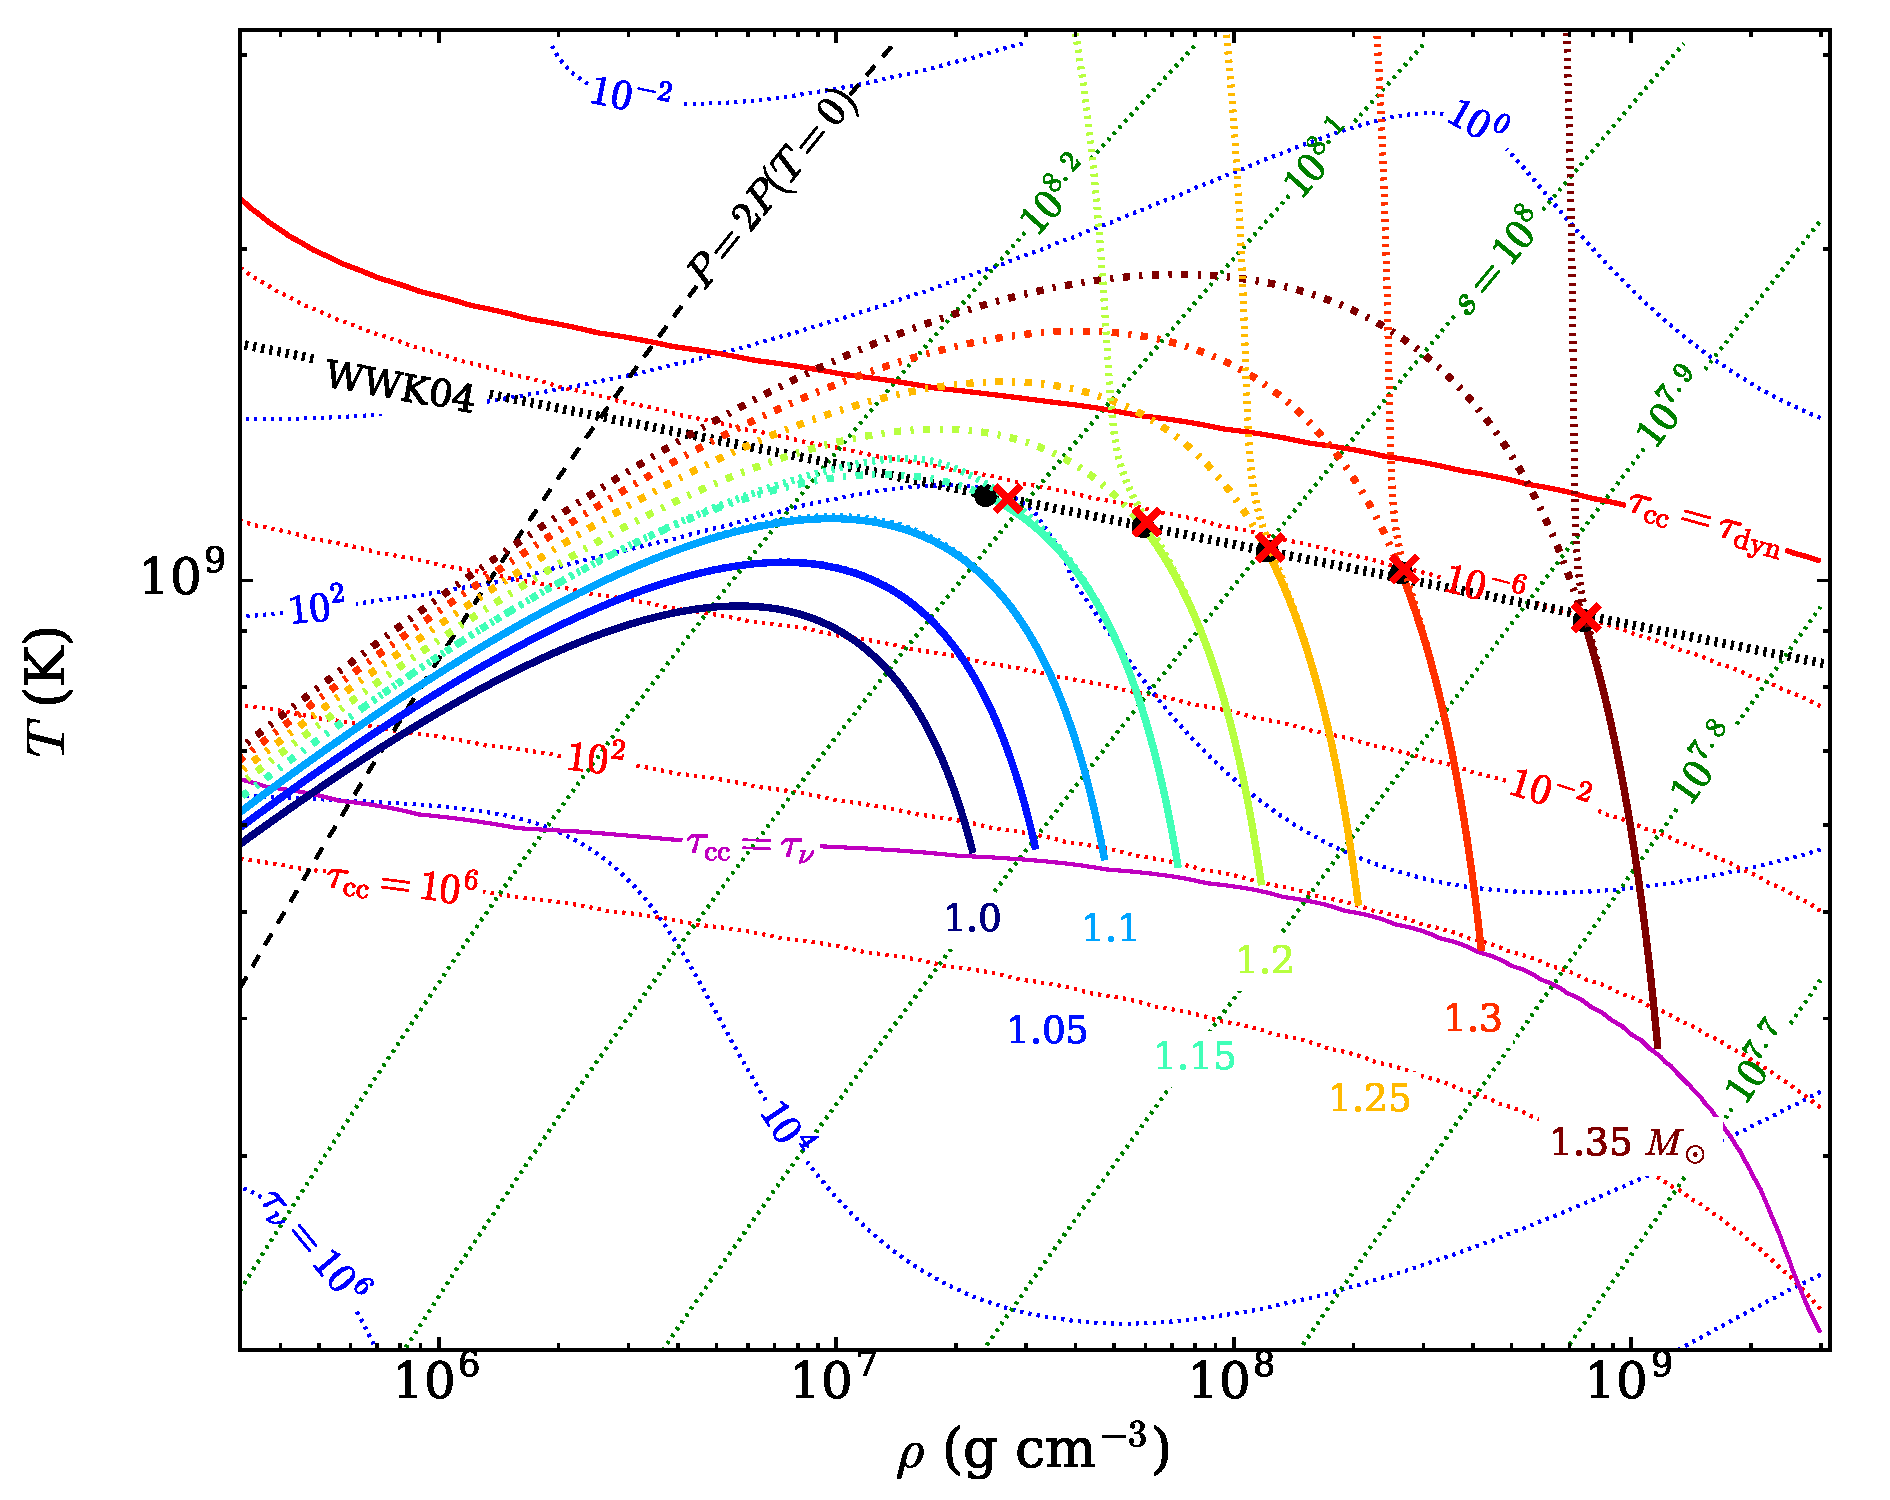
\includegraphics[angle=0,width=1.0\columnwidth]{chapter5_zhu+16/figures/runaway_rhot.pdf}
\caption{Evolution of the central temperature and density -- ``simmering tracks'' -- of simmering CO WDs with masses from $1.0 - 1.35\,\Msun$ (labeled in-line).  Solid lines represent tracks of WDs with adiabatic temperature gradients, with dash-dotted track segments indicating regions that cannot be reached during simmering.  Dotted lines represent tracks that include the superadiabatic deviation \dnabconv\ (Eqn. \ref{eq:c5_superad_dev}) required to transport the convective luminosity.  Black circles along adiabatic simmering tracks indicate ``end of simmering points'' where Eqn. \ref{eq:c5_endofsimmering} is first satisfied, and the black dotted end of simmering line represents a power-law fit to them.  Red Xs are end of simmering points for \dnabconv-inclusive tracks.  Also plotted are contours of constant neutrino cooling timescale \taunu\ and carbon fusion heating timescale \taucc, both in years, as well as specific entropy $s$ in \ergpKg.  The $\taucc = \taunu$ and $\taucc = \taudyn$ lines denote where the fusion heating timescale becomes equal to the neutrino cooling timescale and dynamical timescale (Eqn. \ref{eq:c5_taudyn}), respectively.  Finally, the $P = 2P(T\mrm{=}0)$ approximates the upper bound of the region where degeneracy pressure dominates.  Timescale contours were calculated using \mesa\ \citep{paxt+11}.}
\label{fig:c5_runaway_rhot}
\end{figure}

% Values from papercalc.py/get_adiabatic_numbers()

The simmering tracks roughly form a homology parameterized by a track's highest temperature and a density-axis stretch factor.  Tracks for more massive stars reach higher temperatures and are more horizontally stretched -- the latter is due to entropy being a steeper function of density than degeneracy is when $\rho\gtrsim10^8\,\gcc$ and $T\lesssim10^8\,\mrm{K}$.  The $\taucc = \taunu$ and end of simmering lines, though, reach lower temperatures at higher densities.  As a result, a 1.0 \Msun\ WD is already significantly less degenerate than a 1.35 \Msun\ one at the start of simmering.  At the point where the 1.0 \Msun\ WD reaches its maximum temperature of $9.5\times10^8\,\mrm{K}$ (well short of the end of simmering line), it has expanded considerably, its central density dropping to $\rhoc = 5.6\times10^6\,\gcc$, a quarter of its value at the onset of simmering.  It subsequently continues to expand while cooling.  A 1.35 \Msun\ WD, on the other hand, expands much less drastically -- its central density has decreased by 35\% by its end of simmering point at $\rhoc = 7.6\times10^8\,\gcc$, $\Tc = 9.2\times10^8\,\mrm{K}$.  This central temperature is comparable to the $\Tc = 7-8\times10^8\,\mrm{K}$ commonly reported for the end of simmering for \Mch\ WDs (\citeal{wooswk04}; \citeal{piroc08}).  The convective velocity at the top of the nuclear burning region, $\vconvrcc$, is a few percent of the sound speed $c_s$ at $\Rcc$ for all WDs that reach their end of simmering points; for a 1.15 \Msun\ WD, $\vconvrcc = 1.4\times10^7\,\cmpsec$ ($\sim3$\% of $c_s$), in agreement with our estimate of Eqn. \ref{eq:c5_vconvest2}.

The well-ordered nature of the simmering tracks extends to the end of simmering points, which is why they are well-represented by the end of simmering line.  The line falls just short of the $\taucc = \taudyn$ one, lying just underneath the $\taucc = 10^{-6}\,\mrm{yr}$ contour.  Unlike the other contours in Fig. \ref{fig:c5_runaway_rhot}, this line cannot be calculated independently of the assumptions of the runaway, though we find it is a good approximation for all of our models except for some in Sec. \ref{ssec:c5_rotmag}.

\subsubsection{Estimate of \Mcrit\ and Minimum \MNi}
\label{sssec:c5_mcritest_adiabatic}

We turn to the central task of this paper: estimating the minimum mass \Mcrit\ required to reach the end of simmering point, and the corresponding mass of radioactive nickel \MNi\ produced if an explosion occurs shortly thereafter.  To find \Mcrit, we generated models spaced apart by $0.005\,\Msun$, and find $\Mcrit=1.145\,\Msun$, which ends its simmering with $\rhoc = 2.0\times10^7\,\gcc$, $\Tc = 1.2\times10^9\,\mrm{K}$.

While an explosive event becomes inevitable once the simmering phase ends, its nature -- be it a deflagration, detonation, or some other phenomenon -- has yet to be constrained and is beyond the scope of this work.  We are, however, motivated by the resemblance of pure detonations of sub-\Mch\ WDs to SNe Ia to make a rough estimate of the mass of \Ni, \MNi, produced if the \Mcrit\ WD detonated immediately after simmering ends (i.e. without any further changes to its density structure).  Since a detonation is supersonic, and the input energy for nuclear burning is provided by the shock itself (eg. \citealt{seit+09}), nucleosynthesis in a pure detonation is, to first order, determined by the density profile of the progenitor before the explosion.  Indeed, from the results of \cite{sim+10}, we find that \MNi\ can be estimated to within a few percent by the mass of progenitor material with density $\rho>10^7\,\gcc$, $M(\rho>10^7)$ (see Fig. \ref{fig:c5_mni}).  We can use this simple relationship to estimate that for $\Mcrit = 1.145\,\Msun$, $\MNi = 0.30\,\Msun$.  

Since \Mcrit\ is the minimum mass that can reach the end of simmering point, 0.30 \Msun\ is the minimum amount of \Ni\ produced by any adiabatically simmering WDs (in the absence of either post-simmering expansion or the triggering of a deflagration rather than a detonation).  \MNi, however, rises quite steeply for WDs with $M>\Mcrit$: $M(\rho>10^7) = 0.39\,\Msun$ for a $1.15\,\Msun$ WD, and $0.78\,\Msun$ for a $1.2\,\Msun$ one.  This is because the density of most material in a WD is within an order of magnitude of \rhoc, and \rhoc\ at the end of simmering is a steep function of mass for tracks of $M \approx \Mcrit$, since at that point they run nearly parallel to the end of simmering line.  Therefore, changing \Mcrit\ by a small value, or altering the end of simmering criterion, can substantially change the minimum \MNi.

%and WDs with masses close to \Mcrit\ end simmering with $\rhoc \sim 3\times10^7\,\gcc$,We discuss this further in Sec. \ref{ssec:sensitive}.At this point, its simmering track is nearly parallel to the end of simmering line, suggesting a high degree of sensitivity of \Mcrit\ toward the precise criterion for the end of simmering.  We discuss this further in Sec. \ref{ssec:sensitive}.

\subsubsection{Hot Envelopes}
\label{sssec:c5_runaway_ad_hot}

%(at this temperature, thermal pressure comprises 0.003\% of the total pressure for $\rho = 10^7\,\gcc$)
%We also consider models with ``hot envelopes'' more reminiscent of merger remnants by setting $\tempiso = 2\times10^8\,\mrm{K}$ (thermal pressure is 2\% of the total at $\rho = 1\times10^7\,\gcc$) in Sec. \ref{sssec:runaway_ad_hot}, and find this has a negligible overall effect on the simmering.

%\begin{figure}
%\centering
%\includegraphics[angle=0,width=1.0\columnwidth]{adiabatic_rhot_variation.pdf}
%\caption{Comparison of adiabatic simmering tracks from Fig. \ref{fig:runaway_rhot} (solid lines) with adiabatic ones that have a hot envelope of $\tempiso = 2\times10^8$ K (dashed tracks), and ones that include superadiabatic deviation \dnabconv\ (Eqn. \ref{eq:superad_dev}; dotted lines).  Orange squares represent the end of simmering points for the $\tempiso = 2\times10^8$ K tracks, and cyan inverted triangles represent those for \dnabconv-inclusive ones.  All other lines and symbols are as in Fig. \ref{fig:runaway_rhot}, including the end of simmering line.}
%\label{fig:variations_rhot}
%\end{figure}

% Values from papercalc.py/get_hot_adiabatic_comp() and make_hot_vs_cold_critical()

Fig. \ref{fig:c2_deltamcomp} suggests sub-\Mch\ mergers of WDs with similar mass lead to remnants that are heated throughout, with temperatures between $\sim 1 - 3\times10^8\,\mrm{K}$.  To roughly gauge what effect this pre-runaway heating might have, we generate models identical to the ones above, but set $\tempiso = 2\times10^8\,\mrm{K}$.  We find the simmering tracks of these ``hot-envelope'' WDs deviate most widely from their cold counterparts at the start of simmering, where their central densities are lower by $\sim3-7$\%; these differences reduce to $\sim1 - 6$\% at the end of simmering.  By then, almost the entire interior structure of an adiabatic WD, with \Tc\ $\gtrsim10^9\,\mrm{K}$, has $T > 2\times10^8\,\mrm{K}$, making its central properties insensitive to an increase in \tempiso.  Raising \tempiso\ even further may affect simmering track values more substantially, but hydrostatic solutions of WDs with $\tempiso \gtrsim 5\times10^8\,\mrm{K}$ tend to have low-density atmospheres that extend to arbitrary radii, producing objects of infinite mass.  Any WDs that were heated to such high temperatures by prior evolution, such as the remnant of \cite{ji+13} after its viscous evolution, have more complicated temperature structures that, for simplicity, are not directly considered in this work (see Sec. \ref{ssec:c5_implications} for further discussion).

%  Instead, they are explored in a companion paper \citep{herizv16}.

%The $\sim5$\% ceiling comes from the 1.15 \Msun\ and 1.2 \Msun\ simmering tracks, whose simmering tracks run nearly parallel to the end of simmering line at the end of simmering; the actual shift in \rhoc\ for a 1.15 \Msun\ WD with $\Tc = 1.3\times10^9\,\mrm{K}$ when switching to a hot envelope is $\sim 3$\%.  

\subsection{Superadiabatic Deviation \dnabconv}
\label{ssec:c5_runaway_superad}

To more accurately calculate simmering tracks, we must include the superadiabatic temperature deviation \dnabconv\ (Eqn. \ref{eq:c5_superad_dev}) needed to carry the convective luminosity.  These \dnabconv-inclusive tracks are plotted in Fig. \ref{fig:c5_runaway_rhot} as dotted lines (without indicating track segments unreachable during simmering).  They are, regardless of mass, nearly identical to their adiabatic counterparts during simmering: their \rhoc\ and \Tc\ at the start of simmering match to within floating point precision, and, for WDs of $M > 1.2\Msun$, they also differ by less than 2\% at the end.  While the \dnabconv\ tracks do steepen and arc away from their adiabatic counterparts, this occurs only above their end of simmering points, which are represented by red Xs in Fig. \ref{fig:c5_runaway_rhot} and are well-approximated by the \textit{adiabatic} end of simmering line.  Close to \Mcrit, where the simmering tracks run nearly parallel to the end of simmering line, \dnabconv\ is more influential: the density of the \dnabconv-inclusive 1.15 \Msun\ track at its end of simmering point is $\sim15$\% higher than the adiabatic one.  A mass parameter space search finds $\Mcrit=1.135\,\Msun$, which ends its simmering phase with $\rhoc = 1.7\times10^7\,\gcc$, $\Tc = 1.2\times10^9\,\mrm{K}$.  While these values are very close to the ones obtained in Sec. \ref{sssec:c5_mcritest_adiabatic}, $\MNi = M(\rho>10^7) = 0.20\,\Msun$, which is substantially lower, reflecting its sensitivity to the end of simmering criterion.

%$M(\rho>10^7)$ again rises steeply for WDs with $M>\Mcrit$: $M(\rho>10^7) = 0.45\,\Msun$ for a $1.15\,\Msun$ WD.

The overall tiny effect of \dnabconv\ is due to Eqn. \ref{eq:c5_superad_dev}'s dependence on the square of the ratio of convective velocity to sound speed, $\vconv^2/(g H_P) \approx \vconv^2/c_s^2$.  Like in the adiabatic case, near the end of simmering $(\vconvrcc/c_s(\Rcc))^2 \sim 10^{-3}$ (and $\vconvrcc = 1.3\times10^7\,\cmpsec$) for a $1.15\,\Msun$ WD, and $10^{-4}$ for a $1.35\,\Msun$ one.  This small number is partly offset by the $1/\delta = -d\ln T/d\ln \rho$ term, which approaches infinity for zero-temperature degenerate material.  Near the $\taucc = \taunu$ line, however, the entropy is already sufficiently high that $1/\delta \sim 10^{1.5}$ for a $1.15\,\Msun$ WD, and $\sim 10^{2.5}$ for a $1.35\,\Msun$ one; these values fall to $\sim 10$ and $\sim 10^2$, respectively, near the end of simmering.  Consequently, $\dnabconv \sim 10^{-2}$, an order of magnitude smaller than $\nablaad \approx 0.3 - 0.4$.  Once the end of simmering point is reached, the influence of \dnabconv\ grows to beyond unity at only slightly higher \Sc\ due to the steep dependence of $\vconv^2$ on temperature, resulting in the sharp upward turn in all \dnabconv-inclusive tracks for WDs more massive than $1.2\,\Msun$ in Fig. \ref{fig:c5_runaway_rhot}.

\subsection{Rotation and Magnetic Fields}
\label{ssec:c5_rotmag}

%as well as coupling between rotation, magnetic fields and convection,

We now turn to the inclusion of rotation and magnetic fields, which are expected features of merger remnants.  These, in general, introduce complex multi-dimensional and non-local effects that are challenging to model.  To obtain rough estimates, we consider only uniform rotation or magnetic fields that vary slowly over a convective scale height, ignoring their coupling with each other and with convection, and focus on how either affect \Mcrit.  We first obtain a sense of this effect by estimating the superadiabatic temperature deviation \deltanab\ through energy balance arguments.

In the rotating case, the superadiabatic deviation \dnabrot\ can be estimated by equating the buoyancy and Coriolis forces:

\eqbegin
2\rho\Omega\vconv = -g \left(\frac{d(\Delta \rho)}{dr}\right)\Delta r = g H_P \rho \left(\frac{\delta}{H_P}\dnabrot\right)
\label{eq:c5_dnabrot_est_work}
\eqend

\noindent where $\Delta \rho$ is the density difference between a convective blob and its surroundings and we set the characteristic length of convection $\Delta r$ to $H_P$.  This gives

\eqbegin
\dnabrot = \frac{1}{\delta}\frac{2\Omega H_P}{c_s}\frac{\vconv}{c_s},
\label{eq:c5_dnabrot_est}
\eqend

\noindent where we again use $g H_P \approx c_s^2$.  Eqn. \ref{eq:c5_dnabrot_est} resembles Eqn. \ref{eq:c5_superad_dev}, with one power of $\vconv/c_s$ swapped for $2\Omega H_P/c_s \sim (\Omega^2 H_P/g)^{1/2}$, which is at most $\sim1$ for rotation at break-up.  For our models, $H_P \sim 10^8\,\mrm{cm}$ (as $H_P \sim 1/\alpha$; Sec. \ref{ssec:c5_simmer}) and $g \sim GM_\mrm{WD}/R_\mrm{WD}^2 \sim 10^9\,\cmpsecsq$, so $H_P/g \sim 10^{-1}\,\mathrm{s}^2$.  Also, calculations of remnant viscous evolution \citep{shen+12, schw+12, ji+13} suggest the remnant spins down to well below critical rotation.  $(\Omega^2 H_P/g)^{1/2}$ is therefore more realistically $\lesssim10^{-1}$, and for a $1.15\,\Msun$ WD near the end of simmering, $\dnabrot \lesssim (10^{-1}/\delta)(\vconv/c_s) \sim 10^{-1.5}$, an order of magnitude smaller than \nablaad.  Rotational convective suppression is thus a minor effect.  

In the (non-rotating) magnetized case, we can make a similar estimate by equating the buoyancy and Lorentz forces:

\eqbegin
\frac{B^2}{4\pi H_P} = -g \left(\frac{d(\Delta \rho)}{dr}\right)\Delta r = \rho g \delta \dnabmag,
\label{eq:c5_dnabmag_est_work}
\eqend

\noindent where we use the assumption that the magnetic field varies slowly over $H_P$.  This gives

\eqbegin
\dnabmag = \frac{1}{\delta}\frac{B^2}{4\pi P},
\label{eq:c5_dnabmag_est}
\eqend

\noindent where $\rho g = P/H_P$.  Calculations of magnetic field amplification in mergers (Ch. \ref{ch:ch4}) or during viscous evolution \citep{ji+13} suggest a saturation field strength of $\sim10^{11}\,\mrm{G}$ at the center of the remnant.  Given that $P \gtrsim 10^{25}\,\mrm{dyn\,cm}^{-2}$ at the centers of $\gtrsim 1.15\,\Msun$ WDs, this gives $B^2/4\pi P \lesssim 10^{-4}$, and $\dnabmag \lesssim 10^{-4}/\delta$.  Near the end of simmering, this value is minor (eg. $\sim10^{-3}$ for a $1.15\,\Msun$ WD).

The above suggest that for reasonable rotation rates and magnetic field strengths, their effects on the simmering phase should be small.  To confirm this, we implemented the formulation of \citeauthor{stev79} (\citeyear{stev79}; hereafter \citeal{stev79}), which incorporates rotation and externally imposed magnetic fields (both assumed, as above, to be slowly varying over $H_P$) into Rayleigh-B\'{e}nard convection.  It predicts the convective steady state -- in particular both \deltanab\ and the modified convective velocity -- by finding the growth rates of convective modes using linear stability analysis (\citeal{stev79}, Sec. 2), and then equating them to their non-linear cascade rates, picking the mode with the greatest heat flux to represent the motion as a whole.  While this is \textit{ad hoc}, in the rotation-dominated and unmagnetized limit \citeal{stev79}'s theory reproduces well the convection simulations of \cite{barkdl14} over a wide range of rotation rates.  We summarize our results below; further detail can be found in Sec. \ref{sec:c5_suppression}.

For WDs with sub-critical uniform rotation, we confirm that its effect on simmering is small.  During simmering, \vconv\ increases by orders of magnitude, while $\Omega$ decreases by half an order of magnitude as the WD expands (to conserve angular momentum).  This leads $\Omega H_P/\vconv$ to approach unity, and \dnabrot\ to approach \dnabconv, near the end of simmering for WDs with initial angular speed $\Ominit$ at about a quarter of break up speed \Omcrit.  We also find that $\vconv \propto (\dnabrot/\dnabconv)^{-1/4}$ changes very little, justifying our use of its non-rotating value in the approximation above. For moderate values of $\Omega$, then, simmering tracks shift by only a few percent in density and temperature from their non-rotating versions in Sec. \ref{ssec:c5_runaway_superad}.  When $\Ominit \rightarrow \Omcrit$, Eqn. \ref{eq:c5_dnabrot_est} suggests \dnabrot\ becomes more comparable to \nablaad, but our models show that this is overshadowed by the centrifugal pressure support term in Eqn. \ref{eq:c5_hydroeq}, and the net effect is a reduction of \rhoc\ and \Tc\ for a model with a given \Sc.  This effect increases $\Mcrit$ to $1.14\,\Msun$ for WDs with $\Omega/\Omcrit = 0.5$, though we caution that deviations from spherical symmetry not included in our model become significant near critical rotation.

%\citeal{stev79}'s formulation states that, when the convective kinetic energy density rivals the magnetic energy density, Eqn. \ref{eq:dnabmag_est} should be replaced with Eqn. \ref{eq:superad_dev}, and so for $B \lesssim 3\times10^{11}\,\mrm{G}$ we find \dnabmag\ eventually approaches \dnabconv.

Likewise, we find that simmering tracks for non-rotating WDs with $M\approx\Mcrit$ shift by only a few percent when including magnetic fields.  We choose a field profile that keeps $B^2/P$ constant throughout the WD, and thus can specify a field by its central strength $B(r=0)$.  When performing a parameter-space search for \Mcrit, we alter field strength with mass by keeping the magnetic to total energy ratio of the WD, \EBEtot, fixed.  For $\EBEtot = 2.9\times10^{-5}$, which corresponds to $B(r=0) = 1\times10^{11}\,\mrm{G}$ in a $1.15\,\Msun$ WD at the start of simmering, $\Mcrit = 1.13\,\Msun$.  If we consider field strengths much larger than what is expected for merger remnants, however, we find that, while the simmering track still changes negligibly, the convective velocity \vconv\ becomes proportional to $1/B$ and is dramatically reduced, affecting when Eqn. \ref{eq:c5_endofsimmering} is first satisfied.  A $1.15\,\Msun$ WD threaded by a $B(r=0) = 10^{12}\,\mrm{G}$ field sees its convective velocity reduced by a factor $\sim 10 - 100$, and reaches the end of simmering point at $T = 8\times10^8\,\mrm{K}$, far lower than the (adiabatic) end of simmering line in Fig. \ref{fig:c5_runaway_rhot}.  We determine \Mcrit\ for WDs with $\EBEtot = 2.8\times10^{-3}$, which corresponds to $B(r=0) = 1\times10^{12}\,\mrm{G}$ in a $1.15\,\Msun$ WD at the start of simmering, to be $1.02\,\Msun$, a reduction of more than $0.1\,\Msun$ from the non-magnetized value.

At this strong-field limit, however, the end of simmering point is also well-short of the $\taucc = \taudyn$ line, meaning that a WD that reaches the point must continue to heat up before it can explode.  This heating may eventually lead to an extremely steep temperature gradient that allows for rapid convective energy transport before dynamical burning is reached, but this is beyond the ability for our model to follow.  Moreover, we strongly caution that \citeal{stev79}'s magnetic formulation may not accurately reflect non-linear magnetoconvection, except perhaps in the case of weak fields, and does not include magnetic dynamo processes, which are likely to be efficient in simmering WDs.  We discuss these further in Sec. \ref{ssec:c5_magaccuracy}.

%In the absence of rotation or magnetic fields, \citeal{stev79}'s formulation reproduces Eqns. \ref{eq:vconv_mlt} and \ref{eq:superad_dev}, except with different prefactors, i.e.

%\eqbegin
%\Fconv = 1.66\frac{\rho c_PT}{\gacc\delta} \vconv^3,  %\frac{4\pi}{75}\left(\frac{5}{2}\right)^{5/2}
%\label{eq:vconv_stev_hp}
%\eqend

%\eqbegin
%\dnabconv = 4.57\frac{\vconv^2}{\gacc\delta}\frac{1}{H_P}.
%\label{eq:superad_dev_stev_hp}
%\eqend

%\noindent We tested the effects of using this modified MLT, and find the \dnabconv\ tracks do steepen and arc away from their adiabatic counterparts,
